% !TeX root = ../main.tex

\chapter{Methodology}

\section{Computation Gods}

\paragraph{Q\#1}

We want to have an interacting Hamiltonian
\[
  \mathcal H = \mathcal H_0 + \mathcal V
\]
normally, we consider $\tilde E_0 > \braket<V>$.
\[
  \sum t_{ij} c_i^\dagger c_j + \epsilon_A -2t(\cos kx + \cos ky)
\]
$2Dt = W$. while $V$ energy $u n_\uparrow n_\downarrow$, $W > u$; or $u > W$ is for cookrate. $U \sim \delta t$.
\begin{enumext}
  \item The first thing we will discuss is the Ground State (zero temperature);
  and we also need some thermo equilibrium states (finite $T$), $\rho$: density matrix.
  \item Observables $\Leftrightarrow$ Experiments. $\braket<\hat O>$.
  \begin{itemize}
    \item Thermodynamic: specific head $C_v$; $M$ (magnetisation),
    $\chi$ susceptibility.
    \item Second type of measurement is spectroscopy (Can be transform to many body Green Funcs): it's energy dependent. ARPES means Angel Result . Another called Raman (low frequency). X-ray.
    Using potitros (\textmu-SR); neutron.
  \end{itemize}
\end{enumext}

For MB: $L \to \infty$, $N \to \infty$. infinity | $\braket<x|n>$.

\subparagraph{Q\#1.1}

$\underset\rho{\ket|\Psi>}$: how to represent efficiently? \textrightarrow Quantum Statistical.

For a system: $n$, $T$, $P$, $V$, $\mu$, $S$. Macros
$F(n, \mu, T, ...)$ to get equation of states.

A ``few'' important (enough to determine physical properties)
observables (parameter).
For landau parameters.

\section{How to compute}

\begin{enumerate}
  \item Represent eff.
  \begin{itemize}
    \item Perturbatim, and something beyond that: rariation (functional), mens to minimize sth, ($\delta F$, $\delta E$) to some differential intense Equal group.
    In class method, EL - eq, $\delta L$.
    \begin{itemize}
      \item unperturbed theory ($H_0$): pay attention to degeneracy
      
      quasi-degeneracy (FL), Gapless $\Delta E|_{L\to\infty} \to 0$.
      \item generate perturbation sequences
      
      Feynman diagrem, bookkeeping = wilsm RG.
    \end{itemize}
  \end{itemize}
\end{enumerate}

\section{QM: formulation}

\begin{itemize}
  \item Hamiltonian Mechanics
  \item Lagrangian Mechanins: path integral
\end{itemize}

Pictures (under Hamiltonian)
\begin{itemize}
  \item Schr\"odinger picture
  \item Heisenberg picture
  \item interaction picture (Dirac picture)
\end{itemize}
means where u keep the TIME EVOLUTION.

In Schr\"odinger picture:
\begin{equation}
  \iu\pdv*{}t \ket|\Psi_s(t)> = H\ket|\Psi_s(t)>
\end{equation}
and operators are time-independent.

In Heisenberg picture, states are time-independent.
\[
  -\iu \pdv*{}t \hat O_H(t) = [H, O(t)]
\]
and the relation
\[
  O_H(t) = \upe^{\iu Ht/\hbar} \hat O_p \upe^{-\iu Ht/\hbar}
\]

For Dirac picture, states change slowly
\[
  \iu \pdif t \ket|\Psi_I(t)> = V_I(t) \ket|\Psi_I(t)>
\]
and Evolution accroding to $H$
\[
  -\iu \pdif t O_I(t) = [H_o, O_I(t)]
\]
In some sense, they are equivalent
\[
  O_H(t) = \upe^{\iu Ht/\hbar} \hat O_p \upe^{-\iu Ht/\hbar},~
  O_I(t) = \upe^{\iu Ht/\hbar} \hat O_I \upe^{-\iu Ht/\hbar}
\]

\subsection{Pictures}

Schr\"odinger Picture:
\begin{equation}
  \iu \hbar \pdif t \ket|\psi_s(t)> = H \ket|\psi_s(t)>
\end{equation}
Left: mixed state; Right: $\rho_s$.
$-\iu \hbar\partial_t \rho_s = [H, \rho_s]$

From the above, we derive
\[
  \iu\hbar \pdif t U_s(t,t_0) = H_t U_s(t,t_0)
\]
while $u \sim \upe^{\iu Ht/\hbar}$.

Time evolution operator.
\[
  \ket|\Psi_s(t)> = U_s(t,t_0) \ket|\Psi_s(t_0)>.
\]
and $U^\dagger = U^{-1}$, $U(t_0,t_0) = \identity$.

While $U(t,t_0) = U_s(t,t') U_s(t',t_0)$
\[
  U_s(t,t_0) = 1 - \frac\iu\hbar \int_{t_0}^t \d t_1 H_t \times U_s(t_1,t_0)
\]
So, we can do the following
\[
  U_s(t,t_0) = 1 - \frac\iu\hbar \int_{t_0}^t \d t_1 H_t,~
  U_s(t_1,t_0) = 1 - \frac\iu\hbar \int_{t_0}^{t_1} \d t_2 U(t_1,t_0)
\]
then,
\begin{align*}
  U_s(t,t_0) = 1 - \frac\iu\hbar \int_{t_0}^t \d t_1 H_{t_1}
  \ab(1 - \frac\iu\hbar \int_{t_0}^{t_1} \d t_2 H_{t_2} U(t_0,t_1)) = ...
\end{align*}
equivalent to the equation
\[
  x^2 - x + 1 = 0, ~ x = \frac{-1}{1 - x}
= \frac{-1}{1 - (\frac{-1}{1 - ...})} ~ \text{Continued fraction}
\]
recursion (von Neumann's series)
\begin{equation}
  U_s(t,t_0) = 1 + \sum_{n = 1}^\infty U_s^{(n)} (t,t_0),
\end{equation}
or
\[
  U_s^{(n)}(t,t_0) = \ab(-\frac\iu\hbar)^n \int_{t_0}^{t} \d t_1
  \int_{t_0}^{t_1} \d t_2 \int_{t_0}^{t_2} \d t_3 \cdots \int_{t_0}^{t_{n - 1}} \d t_n \times
  H_{t_1} H_{t_2} \cdots H_{t_n}.
\]
while $t \geq t_1 \geq t_2 \cdots \geq t_n \geq t_0$.

\subsection{Dyson's time-ordering operator}

\[
  T_D(A(t_1) B(t_2)) =
  \begin{cases*}
    A(t_1) B(t_2), & for $t_1 > t_2$\\
    B(t_2) A(t_1), & for $t_2 > t_1$
  \end{cases*}
\]
\begin{center}
  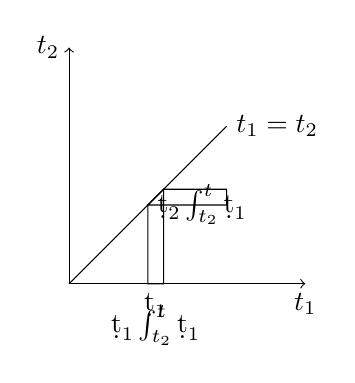
\begin{tikzpicture}
    \draw [->] (0,0) --++ (3,0) node [below] {$t_1$};
    \draw [->] (0,0) --++ (0,3) node [left] {$t_2$};
    \draw (0,0) --++ (2,2) node [right] {$t_1 = t_2$};
    \draw (1,0) -- (1,1) -- (1.2,1.2) -- (1.2,0) -- cycle node [below, midway] {$\d t_1$};
    \node [below = 1ex] at (1.1,0) {$\d t_1 \int_{t_2}^{t} \d t_1$};
    \draw (1,1) -- (2,1) -- (2,1.2) -- (1.2,1.2) -- cycle node [right] {$\d t_2 \int_{t_2}^{t} \d t_1$};
  \end{tikzpicture}
\end{center}
\[
  \d t_2 \int _{t_0}^t \d t_1 \int_{t_0}^{t_1} \d t_2 H_{t_1} H_{t_2}
= \int_{t_3}^{t} \d t_2 \int_{t_2}^t \d t_1 H_{t_1} H_{t_2}
\]
then, $t_1 \Leftrightarrow t_2$
\begin{align*}
  \int_{t_2}^t \d t_1 \int_{t_2}^{t_1} \d t_2 H_{t_1} H_{t_2} &
= \int_{t_0}^t \d t_1 \int_{t_1}^{t} \d t_2 H_{t_2} H_{t_1}\\
& = \frac12 \int_{t_0}^t \d t_1 \int_{t_0}^t \d t
  \ab(H_{t_1} H_{t_2} \theta(t_1 - t_2) + H_{t_2} H_{t_1} \theta(t_2 - t_1))\\
& = \frac1{2!} \int_{t_0}^t \d t_1 \d t_2 T_D(H_{t_1} H_{t_2})
\end{align*}
Generalize
\begin{equation}
  U_s^{(n)}(t,t_0) = \frac1{n!} \ab(-\frac\iu\hbar)^n \int_{t_0}^t \int \d t_1 \cdots \d t_n T_D(H_{t_1} H_{t_2} H_{t_3} \cdots H_{t_n})
\end{equation}
$T_D(H_{t_1}, H_{t_2}, H_{t_3})$:
$\theta(t_1 - t_2)$, $\theta(t_2 - t_1)$,
$\theta(t_2 - t_3)$, $\theta(t_3 - t_2)$,
$\theta(t_3 - t_1)$, $\theta(t_1 - t_3)$, like $2^3 = 8$.
The formal expression
\begin{equation}
  U_s(t,t_0) = T_D \exp\ab(-\frac\iu\hbar \int_{t_0}^t \d t' H_{t'})
\end{equation}

Now, let's try to
\[
  H = H_0 + V
\]

\subsection{Conventional pert}

\begin{gather}
  H_0 \ket|\eta_n> = \eta_n \ket|\eta_n>\\
  H\ket|E_0> = E_0 \ket|E_0>
\end{gather}
while
\[
  \Delta E_0 = E_0 - \eta_0 = \frac{\braket<\eta_0|V|E_0>}{\braket<\eta_0|E>}
\]
where $\ket|E_0> \approx \ket|\eta_0>$.
define $P_0 = \ketbra|\eta_0><\eta_0|$, $Q_0 = 1 - P_0 = \sum_{n=1}^\infty \ketbra|\eta_n><\eta_n|$.
\[
  (D - H_0)\ket|E_0> = (D - \hat H + \hat V) \ket|E_0> = (D - E_0 + \hat V) \ket|E_0>
\]
we get
\begin{equation}
  \ket|E_0> = \frac1{D - H_0} (D - E_0 + V) \ket|E_0>.
= P_0 \ket|E_0> + D_0 \ket|E_0> = \ket|\eta_0>\braket<\eta_0|E_0> + Q_0 \ket|E_0>
\end{equation}
and
\[
  \ket|\tilde E_0> = \frac{\ket|E_0>}{\braket<\eta_0|E_0>}
\]
with this, we can write down the perturbation state
\begin{gather}
  \ket|\tilde E_0> = \ket|\eta_0> + \frac{1}{D - H_0} Q_0 (D - E_0 + V) \ket|\tilde D_0>,\\
  [H_0, P_0] = [Q_0, H_0] = 0,
\end{gather}
while $Q_0$ stands for the projection for orthorgonal basis.
Formally,
\begin{equation}
  \ket|\tilde E_0> = \sum_{m=0}^\infty\ab\{
    \frac{1}{D - H_0} Q_0 (D - E_0 + V)
  \}^m \ket|\eta_0>
\end{equation}
and $\Delta E_0 = \braket<\eta_0|V|\tilde E_0>$.
\begin{itemize}
  \item Schrodinger pert: $D = \eta_0$, $\Delta E_0 (m = 0) = \braket<\eta_0|\lambda v|\eta_0> \sim \lambda$
  \item $\Delta E_0(m = 1) = \frac{\sum|\braket<\eta_0|\lambda v|\eta_n>|^2}{\eta_1 - \eta_n} \sim \lambda^2$, $\Delta E_0(m) \sim \lambda^{m + 1}$.
  \item $\Delta E_0(m = 2) = \sum_{n=1}^\infty \sum_{m=1}^\infty
  \frac{\braket<\eta_0|V|\eta_m> \braket<\eta_m|V|\eta_n>\braket<\eta_n|V|\eta_0>}{(\eta_0 - \eta_m)(\eta_0 - \eta_n)} (\sim \lambda^3)
  - \Delta E_0 \sum\frac{|\braket<\eta_0|V|\eta_n>|^2}{(\eta_0 - \eta_n)^2} (\sim \lambda^2)$
  where $\Delta E_0 \sim (\lambda^0 + \lambda + \cdots + \lambda^m)$.

  $f(\lambda,\lambda^2, \lambda^3)$ mixing $(\lambda^1, \lambda^2, \lambda^3)$.

  interaction problem: diff-integral.
\end{itemize}

\section{Brillouin-Wigner Pert.}

Here, $D = E_0$.

\subsection{Lippmann-Schwinger Equation}

\[
  \hat G = \frac{1}{Z - H_0}, \hat G(z) = \frac1{Z - \hat H}.
\]
we can write
\[
  Z - H_0 = Z - H + V
\]
and
\[
  (1 + V(Z - H)^{-1}) (Z - H) = (1 + \hat V \hat G)(Z - H) = (1 + \hat V \hat G) \hat G^{-1} = (Z - H_0) G
\]
and $G_0^{-1} (Z - H_0) G = 1 + VG$, $\hat G = \hat G_0 + \hat G \hat V \hat G$.
To expand it,
\[
  \hat G = G_0 + G_0 V G_0 + G_0 V G_0 V G_0 + \cdots
\]

\section{Necessity of Gell-Mann-Lon (GML) theorem (No necessity ...)}

Doing sth different
\begin{equation}
  H_\alpha = H_0 + V \upe^{-\alpha |t|}, ~ \alpha > 0
\end{equation}
scuicthing on the interactionL ADIABADIACALLY.
there are two limits,
\begin{gather}
  \lim_{t \to \pm\infty} H_\alpha = H_0;\\
  \lim_{t \to 0} H_\alpha = H
\end{gather}
in the first one, the eigenstate
\[
  \ket|\psi_\alpha(t)> |_{t \to \pm\infty} =
  \begin{cases}
    \ket|\eta_0>, ~ t \to -\infty\\
    e^{\iu\varphi(\alpha)} |\eta_0> t \to \infty
  \end{cases}
\]
for the second one
\[
  \ket|\Psi_\alpha(t)>'|_{t\to0} \to \ket|\Psi_D(t = 0)>,.
\]
and $H\ket|\Psi_D> = E\ket|\Psi_D>$.
as $\alpha > 0$, $\alpha \to 0$, $\pdv*{}\alpha \big|_{\alpha \to 0}$.

\[
  V_D(t) \upe^{-|t|\alpha} = \upe^{\frac1\hbar H_0t} V \upe^{-\frac1\hbar H_0(t)} \upe^{-|t|\alpha}
\]
and we want to compute this: time evolution of:
\begin{equation}
  U_\alpha^D(t,t_0) = \mathcal T_D \upe^{-\frac\iu\hbar \int \d t' V_D(t') \upe^{-|t| \alpha}}
= \sum_{n = 0}^\infty \frac1{n!} \ab(-\frac1\hbar)^n \int_{t_0}^t \int \d t_1 \cdots \d t_n \upe^{-\alpha(|t_1| + \cdots)}
\end{equation}
\[
  T_d \{V_D(t_1), \cdots V_D(t_n)\}
\]
\[
  \ket|\Psi_\alpha^D(t)> = U_\alpha^D (t,t_0) \ket|\Psi_\alpha^D(t_0)> \big|_{t_0 \to \infty}
\]
\begin{enumerate}
  \item $\ket|E_0^D> = \lim_{\alpha\to 0} |\Psi_\alpha^D (0)|_V $ Gell-Mann-Low Theorem
  \[
    \lim_{\alpha \to 0}
    \frac{U_\alpha^D(0,-\infty) \ket|\eta_0>}
      {\braket<\eta_0|U_\alpha^D (0,-\infty)|\eta_0>}
    = \lim_{\alpha\to0}
    \frac{\ket|\Psi_\alpha^D(0)>}{\braket<\eta_0|\Psi_\alpha^D(0)>}
  \]
  so
  \[
    \braket<\eta_0|\Psi_\alpha^D(0)> \xrightarrow{\alpha \to 0}
    \exp\ab(-\iu\frac{f(\lambda)}{\alpha}).
  \]
  Linked-Cluster Theorem
  \begin{align*}
    & \braket<\Psi_\alpha^D(0)| \hat A^D(t)  \hat B^D(t') |\Psi_\alpha^D(0)>\\
  \Rightarrow & \braket<\eta_0|V^D(+\infty,0) \hat A(t) \hat B(t') U_{(0,-\infty)}^D|\eta>\\
  \Rightarrow & \braket<\eta_0|T_D(V^D,\cdots), \hat A(t)\hat B(t')T_D(V^D\cdots)|\eta_0>,\\
  \Rightarrow & F(G_D^{cansal})
  \end{align*}
  From this, we have
  \[
    G^c = \frac{1}{G_v - \epsilon_k^0 - \Sigma}
  \]
  $\ket|\eta_0> \longrightarrow G^c \longrightarrow \ket|\Psi_\alpha^p(0)> \longrightarrow \ket|\eta_0>$ Q:
\end{enumerate}

\section{No-Necssity of GML}

From $\rho_0$: $\ket|\Psi_0>$, $H_0 + \delta H$, to
$\rho = \rho_0 + \delta_\rho$.
To describe MB system more efficientlym we need operator basis (orthogonal, complete) set.
$\{\ket|\eta_n>\}$: inner product. $\Tr[u^\alpha, u^\beta] = \delta^{\alpha\beta}$. $\{u^\alpha\}$ is complete.
\[\hat \rho = \sum u^\alpha \braket<u^\alpha>\]
Fano regonance.
and u find that
\[
  \rho^2 = \rho \Rightarrow \{\rho_0, \delta\rho\} = \delta\rho + \delta\rho^2
\]
so called polynomial eq.

\section{GML \& proof}

\[
  H = H_0 + V\upe^{-\alpha|t|} = H_0 + \lambda\delta H
\]
where $D$ means in Dirac picture
\[
  \lim_{\alpha\to0}
  \frac{u_\alpha^D(0,-\infty) \ket|\eta_0>}{\braket<\eta|u_\alpha^D(0,-\infty)|\eta_0>} = \lim_{\alpha\to0} \frac{\ket|\psi_\alpha^D(0)>}{\braket<\eta_0|\psi_\alpha^D(0)>}
\]
\begin{proof}
  \[
    (H_0 + V) \frac{\ket|\psi_\alpha^D(0)>}{\braket<\eta_0|\psi_\alpha^D(0)>}
= \frac{\braket<\eta_0|H|\psi_0^D(0)>}{\braket<\eta_0|\psi_0^D>}
    \frac{\ket|\psi_\alpha^D(0)>}{\braket<\eta_0|\psi_\alpha^D(0)>}
  \]
\begin{align*}
  (H_0 - \eta_0)\ket|\psi_\alpha^D(0)>
& = -\sum_n \frac1{n!} \ab(-\frac\iu\hbar)^{n-1} \int_{-\infty}^0 \int_{-\infty}^0
  \d t_1 \cdots \d t_n \upe^{-\alpha(|t_1| + \cdots + |t_n|)}\\
& = \cancelto{n\pdv*{}{t_n}}{\ab(\sum_{j=1}^n)} \mathcal T_D (V_D(t_1) V_D(t_2) \cdots V_D(t_n)) \ket|\eta_0>
\end{align*}
  where $\ab(\sum_{j=1}^n \pdv*{}{t_j}) \to n\pdv*{}{t_n}$.
  \begin{center}
  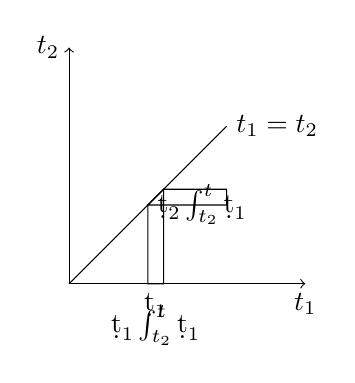
\begin{tikzpicture}
    \draw [->] (0,0) --++ (3,0) node [below] {$t_1$};
    \draw [->] (0,0) --++ (0,3) node [left] {$t_2$};
    \draw (0,0) --++ (2,2) node [right] {$t_1 = t_2$};
    \draw (1,0) -- (1,1) -- (1.2,1.2) -- (1.2,0) -- cycle node [below, midway] {$\d t_1$};
    \node [below = 1ex] at (1.1,0) {$\d t_1 \int_{t_2}^{t} \d t_1$};
    \draw (1,1) -- (2,1) -- (2,1.2) -- (1.2,1.2) -- cycle node [right] {$\d t_2 \int_{t_2}^{t} \d t_1$};
  \end{tikzpicture}
  \end{center}
  $\mathcal T_D(V(t_1) \cdots V(t_n))$
  symmetric of $(t_1 \cdots t_n)$
  it will return corresponding factor due to the order of $t_1t_2t_3 + t_2t_3t_1 + \cdots$
  then u can do integral by part
  
  Causal GFs

  We usually convert
  \[
    \braket<\psi_\alpha^D(0)|\hat a_i^\dagger(t) a_j(t')|\psi_\alpha^D(0)>
  \]
  into Casaul Green Functions
  \[
    G = \frac1{\omega - \epsilon_0 - \Sigma}
  \]
\end{proof}

\subsection{No-Necessity of GML}

Bascially, we can also do perturbation \& variational method.
When given a $H_0$, $\rho_0 + \delta H$
where $\delta\rho = \rho - \rho_0$, and energy $\delta  E$.

Reasit adiabaticity.

route cause: $\ket|\psi> = \frac1{E_0}$
when write into Taylor series: $\ket|\psi(\lambda)> = \ket|\psi_0> + \lambda\ket|\delta\psi> + ...$
and the energy
$E_0(\lambda) = E_0 + \lambda\delta \epsilon^{(1)} + \frac{\lambda^2}{2} \delta \epsilon^{(2)}$
they should be true separate.

There's no need for $E_0$.

In QM: Lippmann-Schwinger
\[
  \hat G = (G_0 - H)^{-1}
\]
But the Lippmann-Schwinger equation we put down is
\[
  \hat G(\omega) = G_0 + G_0VG
\]
diagnal in $\omega$.

As well,
\[
  G(\bm r;\bm r') = G_0(\bm r,\bm r')
- \int \d \bm r'' G_0 (\bm r, \bm r'') \delta V(\bm r'') G(\bm r'',\bm r')
\]
DOES NOT depend on $E_0$.

\section{Complete operator basis set}

wave function $\ket|\Psi> = \upe^{\iu\alpha (...)} = \braket<\hat O>$

``Inner product'' (orthorgonal, completness) $\Tr [\hat u^\alpha, \hat u^\beta] = \delta_{\alpha,\beta}$ C
\[
  \hat O = \sum \braket<u^\alpha>
  \hat o \hat U^\alpha = \sum_\alpha (\bm u^\alpha \cdot \bm O) \bm u^\alpha
\]
where $\braket<>_{\hat O} = \tr[u^\alpha, \hat O]$
\[
  \hat\rho = \sum \braket<\hat u^\alpha> \hat u^\alpha
\]
so we come to some oeelgebraic description
\[
  [\rho,H] = 0
\]
($\otimes$!!! SSB $[\rho, H] \neq 0$)
and the project $\hat \rho^2 = \hat \rho$, with the eigenenergy for pure state condition
\[
  \{\rho, H\} = 2E\hat \rho
\]

* Gerivile to thermal states

$\hat \rho^2 \neq \rho$, but

\subsection{Perturbation theory}

\begin{gather}
  \rho(g) = \rho_0 + g\rho_1 + \frac{g!}{2!}\rho_2\\
  E = E_0 + \delta E = E_0 + gE_1 + \frac{g^2}{2!}E_2 + ...
\end{gather}
$\hat\rho = \hat\rho_0 + \delta\hat\rho$

\[
  \rho^2 = \rho_0^2 + \delta\rho^2 + \{\hat\rho_0,\delta\hat\rho\}
= \hat\rho = \hat\rho_0 + \delta\hat\rho
= \rho_0 + \delta\hat\rho^2 + \{\hat\rho_0, \delta\hat\rho\}
\]
we obtain
\[
  \{\hat\rho_0,\delta\rho\} = \delta\hat\rho - \delta\hat\rho^2
\]
For the Hamiltonian
\[
  H = H_0 + \delta H
\]
the first order term becomes
\[
  O(g'): [\rho_1,H_0] + [\hat\rho_0,\delta H] \approx 0.
\]
then
\[
  \{\hat \rho_0, \hat\rho_1\} = \hat\rho_1
\]
and we have
\[
  [\{\hat\rho_0,\hat\rho_1\}, H_0] + [\hat\rho_0,\delta H] = 0
\]
we expand $\rho_1 = \sum\braket<\hat u^\alpha>_1 \hat u^a$
while $\hat \rho_0 = \sum_{\alpha_0} \braket<u^{\alpha_0}>u^\alpha$
and the trace $\Tr[u^{\alpha}(\text{the equation})] = 0$.
Finally, we get
\[
  \braket<[\delta H, \hat u^{\alpha_0}]> + \sum_\alpha\braket<\{[H_0, \hat u^{\alpha_0}], \hat u^\alpha\}>_0 \braket<u^\alpha>_1 = 0
\]
and we can write it into linear equation
\[
  \hat L \braket<u>_1 + \braket<[\delta H, u^{\alpha_0}]> = 0
\]
where
The $\hat L$ is Liouver super op.
for time evo of $\rho$:
\[
  [H,\delta\rho] = \odv*{\rho}t
= \hat L \rho
\]
More formally,
\[
  [[L_0]] [\rho_1] + [V]_0 = 0
\]
so u can see
\[
  \{\rho_0,\delta\rho\} = \delta\hat\rho - \delta\hat\rho^2
= \delta\hat\rho - \delta\hat\rho(\{\rho_0,\delta\rho\}+\delta\hat\rho^2)
= \delta\hat\rho(1 - \{\rho_0,\delta\rho\}) - \delta\hat\rho^3
\]
concerning the 2nd order term
\[
  O = \braket<[\delta H,u^{\alpha_0}]>_0
    + \sum\delta\braket<u^\alpha>\braket<\{u^\alpha,[H,\hat u^{\alpha_0}]\}>_0
    + \sum_{\gamma\beta} \delta\braket<u^\alpha> \delta \braket<u^\beta>
      \braket<\{u^\gamma, [H,\{u^{\alpha_0}, u^\beta\}]\}>_0 + \cdots
\]
then we start from
$\mathbbm 1 \in co Basis set$. Eq of $\mathbbm 1$, $u^{\alpha_0} = \mathbbm 1$:
\[
  0 = 0 + \sum ...
\]
called linked-cluster-theorem. keep connected term.

In a global form, we can find
\begin{gather*}
  [V]_{0,\alpha_0} + [[L]] \cdot[\delta\hat \rho] + \Tr[\hat u^{\alpha_0}[\delta\hat\rho,H]] = 0\\
  [V] + [[L]][\delta\hat\rho] + [[L_2]][\delta\rho^2] + \Tr[u^{a_0}, [\delta\rho^3,H]]
\end{gather*}
then $L_n$ can be defined as
\[
  L_n \cdot \delta\hat\rho^n = [H,\delta\rho^n]
\]
then
\[
  [V]_0 + \sum_{n=1}^\infty [[L_n]][\delta\rho^n] = 0
\]
then u can get $\delta E$ from $\delta \rho$.

\subsection{Example}

Transversefield Ising model
\[
  H_\text{TFIM} = -J \sum_{ij} S_i^z S_j^z - h_z \sum_i S_i^z = -\delta H - H_0
\]
$\ket|\psi_0> = \ket|\rightarrow\rightarrow\rightarrow \cdots>$
$\rho_0: \braket<S_i^x>_0 = \frac12$, $\braket<SA^\alpha xx>_0 = 0$,
$\braket<S_i^\alpha S_j^\beta>_{C,0} = 0$\footnote{%
  Cumulant: $\braket<S_iS_j>_C
    = \braket<(S_i - \braket<S_i>)(S_j - \braket<S_j>)>$.%
}.
Denote
$u^{\alpha_0} = S_{i0}^y S_{i0+1}^z$
\[
  \braket<[\delta H, n^{\alpha_0}]>_0 \propto \braket<S_i^x S_{i_0+1}^x>_0
\]
we often get
\[
  [H_0, u^{\alpha_0}] = S_{i_e}
\]
\[
  \{u^\alpha,[H_0 u^{\alpha_0}]\} = s_{10}y + S_{i_0+1}^xY + \braket<S^x>_x
\braket<S_x>_z = 0
\]
that is
\[
  \braket<S_i^x,S_{i+1}^x> \sim h/1 g - g_c\big|^{1/8}
\]

2D Heisenberg module

\section{Perturbation}

\subsection{Review of Path Integral in QM}

\[
  \psi(\bm x,t) = \int \d^3x' K(\bm x,t;x',t_0) \psi(\bm x',t_0)
\]
$\braket<x|\psi(t)> \Rightarrow K(\bm x,t;\bm x',t_0) = \braket<\bm x|\upe^{-\iu H(t-t_0)/\hbar}|\bm x'> = \braket<0|\varphi(x,t) \varphi^\dagger(x',t_0)|0>$

PI is based computed on GF directly.
\[
  \sum_{} \upe^{\iu \int_{t,t}^{t,t} L/t}
\]
\[
  \upe^{\iu Ht} \to \upe^{N_i Ht/N} = E^{o}
\]
\[
  \ab(-\frac{\hbar^2}{2m}(\nabla')^2 + V(\bm x) - \iu\hbar\pdv*{}t)
  K(\bm x,t; \bm x_j',t_0)
  = -\iu\hbar\delta^3(\bm x - \bm x')\delta(G-Gaaa)
\]

\subsection{bass Precedures}

\[
  L = L(x,\pdif t, xx, \cdots t)
\]
\begin{itemize}
  \item lassical route
  \item Fluctuations around classic route
\end{itemize}

\subsection{Auadratic Legrangian}

\[
  \psi(x_N, t_\sim, \ket|X_0t_0>)
= \int\d[x(t)] \exp\ab[\frac\iu\hbar S[x,t]]
\]
while consider the Lagrangian
\[
  \mathcal L(x,\dot x,t) = \frac12m\dot x^2 - \frac12 c(t)x^2 - c(t)x
\]
and since $\delta L = 0$, SInce Euler-Lagrangian eq., we have EOM
\[
  m\ddot X_{cl} + c(t) x_{cp} + \upe(t) = 0
\]
then $x(t) = x_{cl}(t) + y(t)$, and
$y(t_0) = y(t_N) = 0$.
then $L(x_{cl}+y,\dot x_{cl} + \dot y,t) = L_{cl}
+ L'(y,\dot y(t), t) + \delta L(\ket|\overset xy>)$
\begin{gather*}
  L_{cl} = \frac12 m\dot x_{cl}^2 - \frac12 c(t) x_{cl} - e(t) x_{cl}\\
  L' = \frac12 m\dot y^2 - \frac12 c(t) y^2
  \delta L = m\dot x_{cl} \dot y(t) - c(t) x_{cl} y - e(t) y
\end{gather*}

\subsection{Perturbation Theory by path integral}

\[
  \dot x_{cl}
 \dot y = \odv*{(\dot x_{cl}y)}t - \ddot x_{cl}y\]
 \[
  \int_{t_0}^{t_N} \d t \delta L = m [\dot x_{cl}y]\bigg|_{t_1}^{t_N}
  - \int_{t_0}^{t_N} (m\ddot x_{cl}(t) + c(t) x_{cl}(t) + e(t)) y(t) \d t
 \]
 then
\[
  \phi(x_N,t_N;x_0,t_0) = \exp\ab\{\frac\iu t S[x_{cl}(t)]\}
  \tilde\phi(0,t_N;0,t_0)
\]
then
\[
  \tilde\phi(0,t_N,0,t_0) = \int_{y(t_0)=d}^{y(t_N) = 0}
  d[y(t_1)] \exp\ab(\frac\iu\hbar \int \d t L')
\]

For discretisaition on $t$:

$\epsilon_N = (t_N - t_0)/N$, and $t_j = t_0 + \epsilon_N j$
\[
  \tilde \phi = \lim_{N \to\infty}
  \ab(\frac{m}{2\pi\iu\hbar\epsilon_0})^{N/2}\times
  \int \d y_1 \d y_2 \cdots \d y_{N-1}
  \exp\ab[\frac\iu\hbar c_N
  \sum\frac12 M\frac{(y_{j+1}-y_j)^2}{\epsilon_N^2} - \frac12 c_jy_j^2]
\]
and the energy $E = \iu\sum y_i a_{jk} y_k$, we have a $(N - 1) \times (N - 1)$ matrix, where $N \to \infty$
\[
  (a_{jk}) = \frac{m}{2\hbar\epsilon_N}
  \begin{pmatrix}
    2 & -1 & ...\\
    -1 & 2 & -1\\
       &  -1 & 2 & ...
  \end{pmatrix}
  -\frac{\epsilon_N}{2\hbar}
  \begin{pmatrix}
    c_1 \\
    & \ddots\\
    & & c_j\\
    & & & \ddots
  \end{pmatrix}
  = \lim_{N \to \infty}
  \ab(\frac{1}{\det[a]})^{1/2}
\]
In the first term of $a_{jk}$, only the diag and two subdiag is non-zero, other elements are zero.

let $D_{N-1} = \det[a]$, then
\[
  D_n = \ab(2 - \frac{\epsilon_N^2}{m}c_N)D_{n-1} - D_{n-2}
\]
and then u get
\[
  D_0 = 1, D_1 = 2 - \frac{\epsilon_N^2}{m}c_1
\]
to the infinite limit,
$\frac{D_{n+1} - 2D_n + D_{n-1}}{\epsilon_N^2} = -\frac{c_{n+1D_n}}{m}$
and when $N \to \infty, \epsilon_N \to 0$,
\[
  \odv[2]{f(t_0,t)}t = -\frac{c(t)}{m}f(t_1,t)
\]
apply the bound condition, show that
\[
  f(t_1,t_0) = 0,
  \odv*{f(t_0,t)}t = 1
\]

\[
  \begin{cases}
    & \phi(xt;x_0t_0) =
    \ab(\frac{m}{2\pi\iu\hbar f(t_0,t)})^{1/2}
    \exp\ab[\frac\iu\hbar S[X_{ct}(t)]],\\
    & \odv[2]{f(t_0,t)}t = -\frac{c(t)}{m} f(t_0,t)
  \end{cases}
\]

For Harmonic Oscillator, $c(t) = m\omega^2$, then
$\ddot f = -\omega^2 f$, so $f(t_0,t) = \sin(\omega(t - t_0))/\omega$.

If consider $\omega \sim \omega_0 + gc(t)$, ...

We are getting $H$, $\epsilon_n$, $\ket|n>$, then we get
$\braket<x|\psi(t)> = \sum_n \underset{\to \upe^{-\epsilon_n\tau/\hbar}}{\braket<x|n>}\upe^{\iu\epsilon_nt/\hbar}$.

To be specifitly,
\[
  \braket<xt|x't'> = \sum_n \varphi_n^*(t) \varphi_n(t') \upe^{-\iu\epsilon_n\Delta t/\hbar}
\]


\subsection{Enclidean Path Integral}

means $t \to i\tau$. Relation to partition func, and spectral repr. decomposition of GFs.
\[
  \braket<x_f,-\iu \tau/2|x_i,\iu\tau/2>\big|_{\tau+\infty}
= \lim_{T\to c_0} \upe^{-E_0T} \varphi_0 (x_f) \varphi_0^*(x_i)
= \braket<x_f|\upe^{-TH}|x_i>
\]

\subsection{Double well problem for PI}

\[
  V(x) = \lambda (x - a)^2
  = \lambda(x-a)^2(x+a)^2
  \sim \lambda(x+a)^2 (2a)^2
  \sim \lambda(x-a)^2 (2a)^2
\]
eigenstates: $\ket|n,+a>$, $\ket|n,-a>$,
$\braket<n_1+a|H|n_1'-a>$
\[
  H' =
  ^^A% \ket|0,+a> & \ket|0,-a>
  \begin{pmatrix}
    H_{a-} & \Delta H\\
    \Delta H & H_{-aa}
  \end{pmatrix}
\]
\begin{enumerate}
  \item $x_{cl}$: $E = 0$. 
  \item $t \to \iu\tau$, the potential $V(x)$, the Lagrangian from $L = T - V$ to $T + V = T - (-V)$, a flipped potential.
  (Why? consider $\upe^{\iu\d t L}$), get $-\dot x^2 -V(x)$, but when $t \to \iu\tau$, u will get $\upe^{-\tau (\dot x^2 -(-V(x)))}$, under the view of Hamiltonian
\end{enumerate}
For 1: $\upe^{\sum x_{cl}}$

For 2: $t\to \infty$, $\upe^{\sum_{EPI}inst}$

\newpage

\section{Apply P.I. for second Quantization}

Begin with the coherent state of H.O..
For Bosons,
\[
  [a_i, a_j^\dagger] = \delta_{ij}
\]
Apply H.O. to Bosons for second quantization.
The eigenstate of the annihilation / creation operator is
\[
  \hat a \ket|\alpha> = \alpha \ket|\alpha>, \qq{but it's wrong that}
  \hat a^\dagger \ket|\alpha> = \alpha \ket|\alpha>
\]
where the coherent state can be expanded in terms of the quantum number state
\[
  \ket|\alpha> = \upe^{-|\alpha|^2/2} \sum \frac{\alpha^n}{\sqrt{n!}} \ket|\varphi_n>
\]
It has some properties
\begin{enumext}
  \item Non-orthogonal
  \begin{equation}
    \braket<\alpha|\alpha'> = \upe^{-|\alpha|^2/2} \upe^{-|\alpha'|^2/2} \upe^{\alpha^*\alpha'}
  \end{equation}
  \item In the quantum number state, we have the identity
  \[
    \sum_n \ketbra|\varphi_n><\varphi_n| = \mathbbm 1,
  \]
  While in the coherent state
  \begin{equation}
    \mathbbm 1 = \frac1\pi \int\ketbra|\alpha><\alpha| \d \Re\alpha \d \Im\alpha
  \end{equation}
  which is overcompleteness.
\end{enumext}

\subsection{Coherentstate of P.I.}

We want to compute
\begin{equation}
  \braket<x|\mathcal U|x'>  = \braket<x| \mathcal T \upe^{\iu H(t - t')}|x'>
= \braket<x|\upe^{\iu\mathcal H\Delta_t} \upe^{\iu\mathcal H\Delta_t} \cdots \upe^{\iu\mathcal H\Delta_t}|x'>
\end{equation}
where $\Delta t = \frac{t - t'}{N}\big|_{N\to\infty}$,
and we can insert the identity $\mathbbm 1$
between the $\upe^{\iu\mathcal H\Delta_t}$s.
Assume for the coherent state $\ket|z>$, we have
\[
  \hat a \ket|z> = z \ket|z>, \quad
  \hat a^\dagger \ket|z> = \pdif z \ket|z>
\]
also for the invert
\[
  \bra<z| \hat a = z \pdif{\bar z} \bra<z|, \quad
  \bra<z| \hat a^\dagger = z \bra<z|,
\]
and we can define
\begin{equation}
  \psi(\bar z) = \braket<z|\psi>, \qq{and}
  \bar \psi(z) = \braket<\psi|z>
\end{equation}
Then the integral can be written as
\begin{equation}
  I = \int \frac{\d z \d \bar z}{2\pi\iu} \upe^{-z\bar z} \ketbra|z><z|
\end{equation}
then, after inserting the identity $\int \frac{\d z(t_n) \d \bar z(t_n)}{2\pi\iu}$, we have
\[
  \cdots \ket|z_{t_{n-1}}>\braket<z_{t_{n-1}}|\exp(\iu\mathcal H(a^\dagger,a)\Delta t)|z_{t_n}|>\bra<z_{t_n}| \upe^{\iu\mathcal H} \cdots
\]
where $\braket<z_{t_{n-1}}|\exp(\iu\mathcal H(a^\dagger,a)\Delta t)|z_{t_n}|>$ is normal ordering, we can rewrite it as
\[
  \braket<z|f(a_i^\dagger a_j^\dagger \cdots a_i a_j)|z'>
= f(\bar z_i, \bar z_j, \cdots z_i, z_j \cdots)
\]
i.e., $a^\dagger \to \bar z$, $a \to z$.
For $\Delta t$, the normal ordering term can be expressed as
\begin{equation}
  \begin{aligned}
    \braket<z_{t_{n-1}}|1 - \frac\iu\hbar \Delta t H(a^\dagger,a)|z_{t_n}>
& = \braket<z_{t_{n-1}}|z_{t_n}>\ab(1 - \frac\iu\hbar \Delta
    \mathcal H(\bar z_{t_{n-1}}, z_{t_n}))\\
& = \upe^{\bar z_{t_{n-1} z_{t_n}}}
    \upe^{-|z_{t_{n-1}}|^2/2} \upe^{-|z_{t_n}|^2/2} (1 - \cdots)\\
& = \int \mathcal D z \mathcal D\bar z
    \exp\ab[\frac\iu\hbar \int_{t_i}^{t_f} \frac\hbar{2\iu} (z\pdif t\bar z - \bar z\pdif t z) - H(\bar z, z)]\\
& = \ldots \exp[\frac12 (|z_i|^2 + |z_f|^2)] \bar \psi_f(z_f) \psi_i(\bar z_i)
  \end{aligned}
\end{equation}

\subsection{Fermionic coherent P.I.}

For the fermions, it satisfy the anti-commutation
\begin{equation}
  \{c_i c_j^\dagger\} = \delta_{ij}, \{c_i, c_j\} = 0
\end{equation}
then for the coherent state, we have
\begin{equation}
  c_i \ket|\xi_i> = \xi_i \ket|\xi_i>,
\end{equation}
where $\ket|\xi_i> = a\ket|0> + b\ket|1>$.
Then, the action can be written into the number state
\begin{equation}
  c \ket|\xi_i> = b_0
\end{equation}
where $b = \xi_i$. We also have the anti-commutator
\begin{equation}
  \{\xi_\alpha, \xi_\beta\} = 0
\end{equation}
We get the Grassmann-variables $\xi_i$, which satisfy
\begin{equation}
  \xi_\alpha^2 = 0, \quad f(\xi_\alpha) = a + b\xi_\alpha, \quad
  \upe^{\xi_\alpha} = 1 + \xi_\alpha, \quad
  \int \d\xi 1 = 0, \int \d\xi \xi = 1,
  \pdv*{(\xi^*)\xi}\xi = \pdv*{-\xi\xi^*}\xi = -\xi^*
\end{equation}
% ^^A \int (t_j \d\xi_i\d\xi_j^*) \upe^{t_j \sum \xi_i^*\xi_j}
We can have the table of Gaussian
$[a_\alpha, a_\beta^\dagger]{-\xi} = \delta_{\alpha\beta}$,
$\ket|\xi> = \upe^\xi \sum_\alpha \xi_\alpha a_\alpha^\dagger\ket|0>$,
$a\ket|\xi> = \xi\ket|\xi>$\\
$\mathbbm 1 = ...$
\begin{equation}
  \int \mathcal D[\xi_\alpha, \xi_\beta^*]
  \exp\ab[-\sum_{\alpha\beta} \xi_\alpha^* \mathcal H_{\alpha\beta}\xi_\beta
  + \sum_\alpha(\eta_\alpha \xi_\alpha^* + \eta_\alpha^* \xi_\alpha)]
  = [\det, \mathcal H]^{-\xi} \sum_{\alpha\beta} \eta_\alpha^* \mathcal H_{\alpha\beta}^{-1} \eta_\beta
\end{equation}
we will discuss later: by taking $\pdv*{}\eta \pdv*{}{\eta^*}$ with $\eta\to 0$ and $\eta^*\to0$ to the expression above.

\subsection{spin-coherent state}

\paragraph{Example}:
Wess-Zumino-Witten term \& Haldane conjecture
with $S^+$, $S^-$, and $\ket|S, \mu>$

We can start from the state
\begin{equation}
  \ket|0> = \ket|SS>, \quad
  S_z\ket|0> = S\ket|0>, \quad
  \hat S^2 \ket|0> = S(S + 1) \ket|0>
\end{equation}
where $S$ is the magnetic number.
The three-dimensional vector $\bm n$
\begin{equation}
  \ket|\bm n> = \upe^{\iu\theta(\bm n_0\times\bm n) \cdot \bm S} \ket|SS>
\end{equation}
where $\bm n \cdot \bm n_0 = \cos\theta$, and $\bm n_0 = (0, 0, 1)$ is a constant vector point to north.
\begin{equation}
  \ket|\bm n> = \sum_{M=-S}^{M=S} \mathcal D(\bm n)_{MS} \ket|SM>
\end{equation}
and the inner product
\begin{equation}
  \braket<\bm n_1|\bm n_2> = \ab[\frac{(1 + \bm n_1 \bm n_2)}2]^S
  \upe^{\iu\Phi(\bm n_1, \bm n_2, \bm n_0)S}
\end{equation}
The vector basis $\{\bm n_i\}$ can be expressed in a Bloch-sphere,
while the identity
\begin{equation}
  \mathbbm 1 = \int \d\mu[\bm n] \ketbra|\bm n><\bm n|
\end{equation}
where
\begin{equation}
  \d \mu(\bm n) = \ab(\frac{2S + 1}{4\pi}) \d^3n \delta(\bm n^2 - 1)
\end{equation}
Now, start from
\[
  \braket<\bm n(t)|\upe^{\iu\Delta t\mathcal H}|\bm n(t_{j+1})>
= \ab(\braket<\bm n(t_j)|\bm n(t_{j+1})>
  + \iu\Delta t\braket<\bm n(t_j)|\mathcal H|\bm n(t_{j+1})>)
\]
and
\[
  \frac{\braket<n(t_j)|\mathcal H|n(t_{j+1})>}{\braket<n(t_j)|n(t_{j+1})>}
  \approxeq \braket<\bm n(t_j)|\mathcal H|\bm n(t_j)> + O(\Delta t)
\]
combine them together
\begin{equation}
  \braket<\bm n(t_j)|\bm n(t_{j+1})> = \upe^{\iu\Phi S}\ab(1 + \frac{\bm n(t_j) \cdot \bm n(t_{j+1})}2)^S
\end{equation}
then we have
\begin{equation}
  \iu S[\bm n] = \iu S \sum_{j=1}^{N_t} \Phi(\bm n_0, \bm n(t_j), \bm n(t_{j+1}))
+ S \sum \ln\ab(1 + \frac{\bm n \cdot \bm n}2) - \braket<n|H|n>
\end{equation}
For a series of magnetic momentum $\bm n(t)$ along a chain,
P.I. to the Hamiltonian is
\[
  \int \d n_i(t) \upe^{\iu J\sum_i \bm S_i \bm S_{i+1}}
\]
and we can see the P.I. approach the phase term
\[
  \frac S2 \underbrace{\int \d t \bm n(t) \cdot (\pdif t \bm n \times \pdif x \bm n)}_{4\pi} = S
\]
For $S = \frac{2n + 1}{2}$, it behaves as a ``crossing'' (X);
when $S = n$, it behaves as a gapped \tikz[scale = .25]{\begin{feynhand}
\vertex (a) at (0,0); \vertex (b) at (2,0);
\propag (a) to [in=90, out=90] (b);
\vertex (c) at (0,1.5); \vertex (d) at (2,1.5);
\propag (c) to [in=-90, out=-90] (d);
\end{feynhand}}.
\[
  I_x \bm S_i^x \bm S_j^x + I_y \bm S_i^x \bm S_j^y
  \longrightarrow S_i^x S_j^- + S_i^- S_j^+ + S^+ S^+ + S^-S^-
\]

\subsection{Review of Methodology \& Source field method}

\begin{enumext}
  \item H-Q.M. GML
  \begin{equation}
    \ket|\Phi> = \mathcal T_0
    \underbrace{\hat S\ket|\Phi_0>}_{\braket<\Phi_0|\mathcal T_0\hat S|\Phi_0>}
  \end{equation}
  Then the inner product
  \begin{equation}
    \braket<\Phi|\mathcal T \psi(1) \psi^\dagger(2)|\Phi>
  = \underbrace{\braket<\Phi|\mathcal T_0 \hat S \psi(1) \psi^\dagger(2)|\Phi_0>}_{\braket<\Phi_0|\mathcal T_0\hat S|\Phi_0>}
  \end{equation}
  The operator $\hat S$ can be expressed as
  \begin{equation}
    \mathcal S = \mathcal T_0 \exp\ab[-\iu\int V(t') \d t'] = \mathcal T_0 \sum_n  (\sim \int \d t_1 \cdots \d t_n)
  \end{equation}
  \item P.I. compute the $S$-matrix scattering 
  \begin{equation}
    \braket<\Phi_0|S|\Phi_0>
  = \int \mathcal D[\psi,\psi^\dagger] \exp\ab(\frac\iu\hbar \int \d t \mathcal L^\text{Gaussian} - V)
  \end{equation}
  we can map $t \to \iu \tau$. The question is how to get
  \begin{equation}
    \braket<\Phi_0|S\psi(1)\psi^\dagger(2)|\Phi_0>
  \end{equation}
  \item $\iu\pdif t \braket<\Psi|\mathcal T_0 \psi(1) \psi^\dagger(2)|\Psi> = \delta [1 - 2] + \braket<|[\psi(1), H]|>$,
  Then we will get the derivative of Green function
  \[
    \iu \pdif t G = \delta[~] + G_k^0 G + \underbrace{\braket<[\psi(1), V], \psi^\dagger(2)>}_\text{Vertex-function}
  \]
  from which we can get \emph{Schr\"odinger-Dyson-EOM}.
  Link through source field method
  \begin{equation}
    H^\text{source} = H + \sum_{t,j} \nu_j(t) \hat\eta \big|_{\nu_\eta(t) \to 0}
  \end{equation}
  Consider add a source of $c$, and $\hat\eta_1 = c_i$, $\hat\eta_2 = c_j^\dagger$. Then we can computer the Green function by taking the functional derivative
  \begin{equation}
    \braket<|c_i(t) c_j^\dagger(t')|>
  = \fdv*{\braket<|\hat S|>}{\nu_{\eta_1}(t), \nu_{\eta_2}(t')}_{\text{source}}
    \big|_{\nu\to0}
  \end{equation}
  we can define
  \begin{equation}
    \Gamma = \braket<\hat O\psi(1); \psi^\dagger(2)> = \fdv*{\braket<\psi(1); \psi^\dagger(2)>}{\nu_{\hat O}}_{\text{Source}} \Big|_{\nu\to 0}
  \end{equation}
  For $H_n = \hat n_\uparrow \hat n_\downarrow$, $\Gamma = u\braket<n_\downarrow(1) c_\uparrow(1); c_\uparrow^\dagger(2)>$. Then the Fourier transformation
  $\mathcal F[\braket<c_\uparrow(1), c_\uparrow^\dagger(2)>]$.

  For exact $G_0$, We can using the skeleton diagram to generate $G_0 + G_0G_\alpha$.

  The Green basically contains
  \begin{equation}
    G[~] = \Delta E_{(n-m)} \braket<\Psi|\psi(x) \psi^\dagger(y)|\psi>,
  \end{equation}
  and $\ket|\Psi>$, $(\rho)$, $\Sigma$.
\end{enumext}